\hypertarget{_geopack__2003_8f}{
\section{/home/mgh/LanlGeoMag/libLanlGeoMag/Geopack\_\-2003.f File Reference}
\label{_geopack__2003_8f}\index{/home/mgh/LanlGeoMag/libLanlGeoMag/Geopack\_\-2003.f@{/home/mgh/LanlGeoMag/libLanlGeoMag/Geopack\_\-2003.f}}
}
\subsection*{Functions}
\begin{CompactItemize}
\item 
subroutine \hyperlink{_geopack__2003_8f_7ed9719f68132703108e5b59d36d7c03}{IGRF\_\-GSM} (XGSM, YGSM, ZGSM, HXGSM, HYGSM, HZGSM)
\item 
subroutine \hyperlink{_geopack__2003_8f_d3225aa14c76ab4531fcf76deb3c15e0}{IGRF\_\-GEO} (R, THETA, PHI, BR, BTHETA, BPHI)
\item 
subroutine \hyperlink{_geopack__2003_8f_a4095b06f000636e34e2581a92ed28f0}{DIP} (XGSM, YGSM, ZGSM, BXGSM, BYGSM, BZGSM)
\item 
subroutine \hyperlink{_geopack__2003_8f_59da55e19c09037b70bd65ec97a3567a}{SUN} (IYEAR, IDAY, IHOUR, MINUTE, ISEC, GST, SLONG, SRASN, SDEC)
\item 
subroutine \hyperlink{_geopack__2003_8f_51cbeafec4591bc974f865375cec3975}{SPHCAR} (R, THETA, PHI, X, Y, Z, J)
\item 
subroutine \hyperlink{_geopack__2003_8f_39f847a454b8691795bb0b0421de3a70}{BSPCAR} (THETA, PHI, BR, BTHETA, BPHI, BX, BY, BZ)
\item 
subroutine \hyperlink{_geopack__2003_8f_96aa3aaadaaa8312679747d9c48e3b51}{BCARSP} (X, Y, Z, BX, BY, BZ, BR, BTHETA, BPHI)
\item 
subroutine \hyperlink{_geopack__2003_8f_57fa81f55e16b42ac170dbf64e99a5b4}{RECALC} (IYEAR, IDAY, IHOUR, MINUTE, ISEC)
\item 
subroutine \hyperlink{_geopack__2003_8f_e0b60382c97039de9f797a776af33eb7}{GEOMAG} (XGEO, YGEO, ZGEO, XMAG, YMAG, ZMAG, J)
\item 
subroutine \hyperlink{_geopack__2003_8f_eacac87be2a894945521bf5ef2f9ef56}{GEIGEO} (XGEI, YGEI, ZGEI, XGEO, YGEO, ZGEO, J)
\item 
subroutine \hyperlink{_geopack__2003_8f_f5577c4fb7c2ae0b88ab96b884780760}{MAGSM} (XMAG, YMAG, ZMAG, XSM, YSM, ZSM, J)
\item 
subroutine \hyperlink{_geopack__2003_8f_44cb43398834cd0273a73264ea6e7057}{GSMGSE} (XGSM, YGSM, ZGSM, XGSE, YGSE, ZGSE, J)
\item 
subroutine \hyperlink{_geopack__2003_8f_3c1b6bd041138ad15b19a284572c0283}{SMGSM} (XSM, YSM, ZSM, XGSM, YGSM, ZGSM, J)
\item 
subroutine \hyperlink{_geopack__2003_8f_a724192dda005c0ef8d4e8cb9d5465dd}{GEOGSM} (XGEO, YGEO, ZGEO, XGSM, YGSM, ZGSM, J)
\item 
subroutine \hyperlink{_geopack__2003_8f_964ce3d6c1eb16a70ec41d33544e4d07}{RHAND} (X, Y, Z, R1, R2, R3, IOPT, PARMOD, EXNAME, INNAME)
\item 
subroutine \hyperlink{_geopack__2003_8f_4b84b9909d3de37b1cbfd0e8ef98d2af}{STEP} (X, Y, Z, DS, ERRIN, IOPT, PARMOD, EXNAME, INNAME)
\item 
subroutine \hyperlink{_geopack__2003_8f_e88b362d0d3c99ad9c733e9fc088b731}{TRACE} (XI, YI, ZI, DIR, RLIM, R0, IOPT, PARMOD, EXNAME, INNAME,$\ast$XF, YF, ZF, XX, YY, ZZ, L)
\item 
subroutine \hyperlink{_geopack__2003_8f_3bab20b0a7497f74438bdbad9bd01271}{SHUETAL\_\-MGNP} (XN\_\-PD, VEL, BZIMF, XGSM, YGSM, ZGSM,$\ast$XMGNP, YMGNP, ZMGNP, DIST, ID)
\item 
subroutine \hyperlink{_geopack__2003_8f_eb78a92a9deaca0077c026b5adf32cad}{T96\_\-MGNP} (XN\_\-PD, VEL, XGSM, YGSM, ZGSM, XMGNP, YMGNP, ZMGNP,$\ast$DIST, ID)
\end{CompactItemize}


\subsection{Function Documentation}
\hypertarget{_geopack__2003_8f_7ed9719f68132703108e5b59d36d7c03}{
\index{Geopack\_\-2003.f@{Geopack\_\-2003.f}!IGRF\_\-GSM@{IGRF\_\-GSM}}
\index{IGRF\_\-GSM@{IGRF\_\-GSM}!Geopack_2003.f@{Geopack\_\-2003.f}}
\subsubsection[{IGRF\_\-GSM}]{\setlength{\rightskip}{0pt plus 5cm}subroutine IGRF\_\-GSM (XGSM, \/  YGSM, \/  ZGSM, \/  HXGSM, \/  HYGSM, \/  HZGSM)}}
\label{_geopack__2003_8f_7ed9719f68132703108e5b59d36d7c03}




Definition at line 87 of file Geopack\_\-2003.f.

Here is the call graph for this function:\nopagebreak
\begin{figure}[H]
\begin{center}
\leavevmode
\includegraphics[width=104pt]{_geopack__2003_8f_7ed9719f68132703108e5b59d36d7c03_cgraph}
\end{center}
\end{figure}
\hypertarget{_geopack__2003_8f_d3225aa14c76ab4531fcf76deb3c15e0}{
\index{Geopack\_\-2003.f@{Geopack\_\-2003.f}!IGRF\_\-GEO@{IGRF\_\-GEO}}
\index{IGRF\_\-GEO@{IGRF\_\-GEO}!Geopack_2003.f@{Geopack\_\-2003.f}}
\subsubsection[{IGRF\_\-GEO}]{\setlength{\rightskip}{0pt plus 5cm}subroutine IGRF\_\-GEO (R, \/  THETA, \/  PHI, \/  BR, \/  BTHETA, \/  BPHI)}}
\label{_geopack__2003_8f_d3225aa14c76ab4531fcf76deb3c15e0}




Definition at line 214 of file Geopack\_\-2003.f.\hypertarget{_geopack__2003_8f_a4095b06f000636e34e2581a92ed28f0}{
\index{Geopack\_\-2003.f@{Geopack\_\-2003.f}!DIP@{DIP}}
\index{DIP@{DIP}!Geopack_2003.f@{Geopack\_\-2003.f}}
\subsubsection[{DIP}]{\setlength{\rightskip}{0pt plus 5cm}subroutine DIP (XGSM, \/  YGSM, \/  ZGSM, \/  BXGSM, \/  BYGSM, \/  BZGSM)}}
\label{_geopack__2003_8f_a4095b06f000636e34e2581a92ed28f0}




Definition at line 325 of file Geopack\_\-2003.f.\hypertarget{_geopack__2003_8f_59da55e19c09037b70bd65ec97a3567a}{
\index{Geopack\_\-2003.f@{Geopack\_\-2003.f}!SUN@{SUN}}
\index{SUN@{SUN}!Geopack_2003.f@{Geopack\_\-2003.f}}
\subsubsection[{SUN}]{\setlength{\rightskip}{0pt plus 5cm}subroutine SUN (IYEAR, \/  IDAY, \/  IHOUR, \/  MINUTE, \/  ISEC, \/  GST, \/  SLONG, \/  SRASN, \/  SDEC)}}
\label{_geopack__2003_8f_59da55e19c09037b70bd65ec97a3567a}




Definition at line 358 of file Geopack\_\-2003.f.

Here is the caller graph for this function:\nopagebreak
\begin{figure}[H]
\begin{center}
\leavevmode
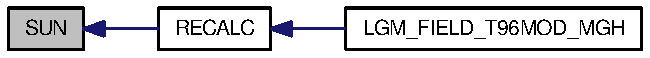
\includegraphics[width=174pt]{_geopack__2003_8f_59da55e19c09037b70bd65ec97a3567a_icgraph}
\end{center}
\end{figure}
\hypertarget{_geopack__2003_8f_51cbeafec4591bc974f865375cec3975}{
\index{Geopack\_\-2003.f@{Geopack\_\-2003.f}!SPHCAR@{SPHCAR}}
\index{SPHCAR@{SPHCAR}!Geopack_2003.f@{Geopack\_\-2003.f}}
\subsubsection[{SPHCAR}]{\setlength{\rightskip}{0pt plus 5cm}subroutine SPHCAR (R, \/  THETA, \/  PHI, \/  X, \/  Y, \/  Z, \/  J)}}
\label{_geopack__2003_8f_51cbeafec4591bc974f865375cec3975}




Definition at line 408 of file Geopack\_\-2003.f.\hypertarget{_geopack__2003_8f_39f847a454b8691795bb0b0421de3a70}{
\index{Geopack\_\-2003.f@{Geopack\_\-2003.f}!BSPCAR@{BSPCAR}}
\index{BSPCAR@{BSPCAR}!Geopack_2003.f@{Geopack\_\-2003.f}}
\subsubsection[{BSPCAR}]{\setlength{\rightskip}{0pt plus 5cm}subroutine BSPCAR (THETA, \/  PHI, \/  BR, \/  BTHETA, \/  BPHI, \/  BX, \/  BY, \/  BZ)}}
\label{_geopack__2003_8f_39f847a454b8691795bb0b0421de3a70}




Definition at line 450 of file Geopack\_\-2003.f.\hypertarget{_geopack__2003_8f_96aa3aaadaaa8312679747d9c48e3b51}{
\index{Geopack\_\-2003.f@{Geopack\_\-2003.f}!BCARSP@{BCARSP}}
\index{BCARSP@{BCARSP}!Geopack_2003.f@{Geopack\_\-2003.f}}
\subsubsection[{BCARSP}]{\setlength{\rightskip}{0pt plus 5cm}subroutine BCARSP (X, \/  Y, \/  Z, \/  BX, \/  BY, \/  BZ, \/  BR, \/  BTHETA, \/  BPHI)}}
\label{_geopack__2003_8f_96aa3aaadaaa8312679747d9c48e3b51}




Definition at line 475 of file Geopack\_\-2003.f.\hypertarget{_geopack__2003_8f_57fa81f55e16b42ac170dbf64e99a5b4}{
\index{Geopack\_\-2003.f@{Geopack\_\-2003.f}!RECALC@{RECALC}}
\index{RECALC@{RECALC}!Geopack_2003.f@{Geopack\_\-2003.f}}
\subsubsection[{RECALC}]{\setlength{\rightskip}{0pt plus 5cm}subroutine RECALC (IYEAR, \/  IDAY, \/  IHOUR, \/  MINUTE, \/  ISEC)}}
\label{_geopack__2003_8f_57fa81f55e16b42ac170dbf64e99a5b4}




Definition at line 514 of file Geopack\_\-2003.f.

Here is the call graph for this function:\nopagebreak
\begin{figure}[H]
\begin{center}
\leavevmode
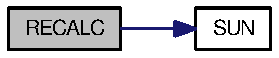
\includegraphics[width=85pt]{_geopack__2003_8f_57fa81f55e16b42ac170dbf64e99a5b4_cgraph}
\end{center}
\end{figure}


Here is the caller graph for this function:\nopagebreak
\begin{figure}[H]
\begin{center}
\leavevmode

\includegraphics[width=138pt]{_geopack__2003_8f_57fa81f55e16b42ac170dbf64e99a5b4_icgraph}
\end{center}
\end{figure}
\hypertarget{_geopack__2003_8f_e0b60382c97039de9f797a776af33eb7}{
\index{Geopack\_\-2003.f@{Geopack\_\-2003.f}!GEOMAG@{GEOMAG}}
\index{GEOMAG@{GEOMAG}!Geopack_2003.f@{Geopack\_\-2003.f}}
\subsubsection[{GEOMAG}]{\setlength{\rightskip}{0pt plus 5cm}subroutine GEOMAG (XGEO, \/  YGEO, \/  ZGEO, \/  XMAG, \/  YMAG, \/  ZMAG, \/  J)}}
\label{_geopack__2003_8f_e0b60382c97039de9f797a776af33eb7}




Definition at line 981 of file Geopack\_\-2003.f.\hypertarget{_geopack__2003_8f_eacac87be2a894945521bf5ef2f9ef56}{
\index{Geopack\_\-2003.f@{Geopack\_\-2003.f}!GEIGEO@{GEIGEO}}
\index{GEIGEO@{GEIGEO}!Geopack_2003.f@{Geopack\_\-2003.f}}
\subsubsection[{GEIGEO}]{\setlength{\rightskip}{0pt plus 5cm}subroutine GEIGEO (XGEI, \/  YGEI, \/  ZGEI, \/  XGEO, \/  YGEO, \/  ZGEO, \/  J)}}
\label{_geopack__2003_8f_eacac87be2a894945521bf5ef2f9ef56}




Definition at line 1017 of file Geopack\_\-2003.f.\hypertarget{_geopack__2003_8f_f5577c4fb7c2ae0b88ab96b884780760}{
\index{Geopack\_\-2003.f@{Geopack\_\-2003.f}!MAGSM@{MAGSM}}
\index{MAGSM@{MAGSM}!Geopack_2003.f@{Geopack\_\-2003.f}}
\subsubsection[{MAGSM}]{\setlength{\rightskip}{0pt plus 5cm}subroutine MAGSM (XMAG, \/  YMAG, \/  ZMAG, \/  XSM, \/  YSM, \/  ZSM, \/  J)}}
\label{_geopack__2003_8f_f5577c4fb7c2ae0b88ab96b884780760}




Definition at line 1051 of file Geopack\_\-2003.f.\hypertarget{_geopack__2003_8f_44cb43398834cd0273a73264ea6e7057}{
\index{Geopack\_\-2003.f@{Geopack\_\-2003.f}!GSMGSE@{GSMGSE}}
\index{GSMGSE@{GSMGSE}!Geopack_2003.f@{Geopack\_\-2003.f}}
\subsubsection[{GSMGSE}]{\setlength{\rightskip}{0pt plus 5cm}subroutine GSMGSE (XGSM, \/  YGSM, \/  ZGSM, \/  XGSE, \/  YGSE, \/  ZGSE, \/  J)}}
\label{_geopack__2003_8f_44cb43398834cd0273a73264ea6e7057}




Definition at line 1085 of file Geopack\_\-2003.f.\hypertarget{_geopack__2003_8f_3c1b6bd041138ad15b19a284572c0283}{
\index{Geopack\_\-2003.f@{Geopack\_\-2003.f}!SMGSM@{SMGSM}}
\index{SMGSM@{SMGSM}!Geopack_2003.f@{Geopack\_\-2003.f}}
\subsubsection[{SMGSM}]{\setlength{\rightskip}{0pt plus 5cm}subroutine SMGSM (XSM, \/  YSM, \/  ZSM, \/  XGSM, \/  YGSM, \/  ZGSM, \/  J)}}
\label{_geopack__2003_8f_3c1b6bd041138ad15b19a284572c0283}




Definition at line 1119 of file Geopack\_\-2003.f.\hypertarget{_geopack__2003_8f_a724192dda005c0ef8d4e8cb9d5465dd}{
\index{Geopack\_\-2003.f@{Geopack\_\-2003.f}!GEOGSM@{GEOGSM}}
\index{GEOGSM@{GEOGSM}!Geopack_2003.f@{Geopack\_\-2003.f}}
\subsubsection[{GEOGSM}]{\setlength{\rightskip}{0pt plus 5cm}subroutine GEOGSM (XGEO, \/  YGEO, \/  ZGEO, \/  XGSM, \/  YGSM, \/  ZGSM, \/  J)}}
\label{_geopack__2003_8f_a724192dda005c0ef8d4e8cb9d5465dd}




Definition at line 1153 of file Geopack\_\-2003.f.

Here is the caller graph for this function:\nopagebreak
\begin{figure}[H]
\begin{center}
\leavevmode
\includegraphics[width=104pt]{_geopack__2003_8f_a724192dda005c0ef8d4e8cb9d5465dd_icgraph}
\end{center}
\end{figure}
\hypertarget{_geopack__2003_8f_964ce3d6c1eb16a70ec41d33544e4d07}{
\index{Geopack\_\-2003.f@{Geopack\_\-2003.f}!RHAND@{RHAND}}
\index{RHAND@{RHAND}!Geopack_2003.f@{Geopack\_\-2003.f}}
\subsubsection[{RHAND}]{\setlength{\rightskip}{0pt plus 5cm}subroutine RHAND (X, \/  Y, \/  Z, \/  R1, \/  R2, \/  R3, \/  IOPT, \/  PARMOD, \/  EXNAME, \/  INNAME)}}
\label{_geopack__2003_8f_964ce3d6c1eb16a70ec41d33544e4d07}




Definition at line 1188 of file Geopack\_\-2003.f.

Here is the caller graph for this function:\nopagebreak
\begin{figure}[H]
\begin{center}
\leavevmode
\includegraphics[width=129pt]{_geopack__2003_8f_964ce3d6c1eb16a70ec41d33544e4d07_icgraph}
\end{center}
\end{figure}
\hypertarget{_geopack__2003_8f_4b84b9909d3de37b1cbfd0e8ef98d2af}{
\index{Geopack\_\-2003.f@{Geopack\_\-2003.f}!STEP@{STEP}}
\index{STEP@{STEP}!Geopack_2003.f@{Geopack\_\-2003.f}}
\subsubsection[{STEP}]{\setlength{\rightskip}{0pt plus 5cm}subroutine STEP (X, \/  Y, \/  Z, \/  DS, \/  ERRIN, \/  IOPT, \/  PARMOD, \/  EXNAME, \/  INNAME)}}
\label{_geopack__2003_8f_4b84b9909d3de37b1cbfd0e8ef98d2af}




Definition at line 1220 of file Geopack\_\-2003.f.

Here is the call graph for this function:\nopagebreak
\begin{figure}[H]
\begin{center}
\leavevmode
\includegraphics[width=86pt]{_geopack__2003_8f_4b84b9909d3de37b1cbfd0e8ef98d2af_cgraph}
\end{center}
\end{figure}


Here is the caller graph for this function:\nopagebreak
\begin{figure}[H]
\begin{center}
\leavevmode
\includegraphics[width=86pt]{_geopack__2003_8f_4b84b9909d3de37b1cbfd0e8ef98d2af_icgraph}
\end{center}
\end{figure}
\hypertarget{_geopack__2003_8f_e88b362d0d3c99ad9c733e9fc088b731}{
\index{Geopack\_\-2003.f@{Geopack\_\-2003.f}!TRACE@{TRACE}}
\index{TRACE@{TRACE}!Geopack_2003.f@{Geopack\_\-2003.f}}
\subsubsection[{TRACE}]{\setlength{\rightskip}{0pt plus 5cm}subroutine TRACE (XI, \/  YI, \/  ZI, \/  DIR, \/  RLIM, \/  R0, \/  IOPT, \/  PARMOD, \/  EXNAME, \/  INNAME, \/  $\ast$ {\em XF}, \/  YF, \/  ZF, \/  XX, \/  YY, \/  ZZ, \/  L)}}
\label{_geopack__2003_8f_e88b362d0d3c99ad9c733e9fc088b731}




Definition at line 1264 of file Geopack\_\-2003.f.

Here is the call graph for this function:\nopagebreak
\begin{figure}[H]
\begin{center}
\leavevmode
\includegraphics[width=129pt]{_geopack__2003_8f_e88b362d0d3c99ad9c733e9fc088b731_cgraph}
\end{center}
\end{figure}
\hypertarget{_geopack__2003_8f_3bab20b0a7497f74438bdbad9bd01271}{
\index{Geopack\_\-2003.f@{Geopack\_\-2003.f}!SHUETAL\_\-MGNP@{SHUETAL\_\-MGNP}}
\index{SHUETAL\_\-MGNP@{SHUETAL\_\-MGNP}!Geopack_2003.f@{Geopack\_\-2003.f}}
\subsubsection[{SHUETAL\_\-MGNP}]{\setlength{\rightskip}{0pt plus 5cm}subroutine SHUETAL\_\-MGNP (XN\_\-PD, \/  VEL, \/  BZIMF, \/  XGSM, \/  YGSM, \/  ZGSM, \/  $\ast$ {\em XMGNP}, \/  YMGNP, \/  ZMGNP, \/  DIST, \/  ID)}}
\label{_geopack__2003_8f_3bab20b0a7497f74438bdbad9bd01271}




Definition at line 1416 of file Geopack\_\-2003.f.

Here is the call graph for this function:\nopagebreak
\begin{figure}[H]
\begin{center}
\leavevmode
\includegraphics[width=160pt]{_geopack__2003_8f_3bab20b0a7497f74438bdbad9bd01271_cgraph}
\end{center}
\end{figure}
\hypertarget{_geopack__2003_8f_eb78a92a9deaca0077c026b5adf32cad}{
\index{Geopack\_\-2003.f@{Geopack\_\-2003.f}!T96\_\-MGNP@{T96\_\-MGNP}}
\index{T96\_\-MGNP@{T96\_\-MGNP}!Geopack_2003.f@{Geopack\_\-2003.f}}
\subsubsection[{T96\_\-MGNP}]{\setlength{\rightskip}{0pt plus 5cm}subroutine T96\_\-MGNP (XN\_\-PD, \/  VEL, \/  XGSM, \/  YGSM, \/  ZGSM, \/  XMGNP, \/  YMGNP, \/  ZMGNP, \/  $\ast$ {\em DIST}, \/  ID)}}
\label{_geopack__2003_8f_eb78a92a9deaca0077c026b5adf32cad}




Definition at line 1535 of file Geopack\_\-2003.f.

Here is the call graph for this function:\nopagebreak
\begin{figure}[H]
\begin{center}
\leavevmode
\includegraphics[width=94pt]{_geopack__2003_8f_eb78a92a9deaca0077c026b5adf32cad_cgraph}
\end{center}
\end{figure}


Here is the caller graph for this function:\nopagebreak
\begin{figure}[H]
\begin{center}
\leavevmode
\includegraphics[width=122pt]{_geopack__2003_8f_eb78a92a9deaca0077c026b5adf32cad_icgraph}
\end{center}
\end{figure}
